% This template has been tested with IEEEtran of 2015.

% !TeX spellcheck = en-US
% LTeX: language=en-US
% !TeX encoding = utf8
% !TeX program = pdflatex
% !BIB program = bibtex
% -*- coding:utf-8 mod:LaTeX -*-

% DO NOT DOWNLOAD IEEEtran.cls - Use the one of your LaTeX distribution
% For the final version, replace "draftcls" by "final"
\documentclass[conference,a4paper,english]{IEEEtran}[2015/08/26]

% Balance the last page using the balance package (see https://ctan.org/pkg/balance)
% Alternative to balance is the pbalance package (see https://ctan.org/pkg/pbalance), which sometimes works better
\usepackage{balance}

% backticks (`) are rendered as such in verbatim environments.
% See following links for details:
%   - https://tex.stackexchange.com/a/341057/9075
%   - https://tex.stackexchange.com/a/47451/9075
%   - https://tex.stackexchange.com/a/166791/9075
\usepackage{upquote}

% Set English as language and allow to write hyphenated"=words
%
% Even though `american`, `english` and `USenglish` are synonyms for babel package (according to https://tex.stackexchange.com/questions/12775/babel-english-american-usenglish), the llncs document class is prepared to avoid the overriding of certain names (such as "Abstract." -> "Abstract" or "Fig." -> "Figure") when using `english`, but not when using the other 2.
% english has to go last to set it as default language
\usepackage[ngerman,main=english]{babel}
%
% Hint by http://tex.stackexchange.com/a/321066/9075 -> enable "= as dashes
\addto\extrasenglish{\languageshorthands{ngerman}\useshorthands{"}}

% Links behave as they should. Enables "\url{...}" for URL typesettings.
% Allow URL breaks also at a hyphen, even though it might be confusing: Is the "-" part of the address or just a hyphen?
% See https://tex.stackexchange.com/a/3034/9075.
\usepackage[hyphens]{url}

% When activated, use text font as url font, not the monospaced one.
% For all options see https://tex.stackexchange.com/a/261435/9075.
% \urlstyle{same}

% Improve wrapping of URLs - hint by http://tex.stackexchange.com/a/10419/9075
\makeatletter
\g@addto@macro{\UrlBreaks}{\UrlOrds}
\makeatother

% nicer // - solution by http://tex.stackexchange.com/a/98470/9075
% DO NOT ACTIVATE -> prevents line breaks
%\makeatletter
%\def\Url@twoslashes{\mathchar`\/\@ifnextchar/{\kern-.2em}{}}
%\g@addto@macro\UrlSpecials{\do\/{\Url@twoslashes}}
%\makeatother


% use nicer font for code
\usepackage[zerostyle=b,scaled=.75]{newtxtt}

% Has to be loaded AFTER any font packages. See https://tex.stackexchange.com/a/2869/9075.
\usepackage[T1]{fontenc}
\usepackage{algorithmic}

% Character protrusion and font expansion. See http://www.ctan.org/tex-archive/macros/latex/contrib/microtype/

\usepackage[
  babel=true, % Enable language-specific kerning. Take language-settings from the languge of the current document (see Section 6 of microtype.pdf)
  expansion=alltext,
  protrusion=alltext-nott, % Ensure that at listings, there is no change at the margin of the listing
  final % Always enable microtype, even if in draft mode. This helps finding bad boxes quickly.
        % In the standard configuration, this template is always in the final mode, so this option only makes a difference if "pros" use the draft mode
]{microtype}

% \texttt{test -- test} keeps the "--" as "--" (and does not convert it to an en dash)
\DisableLigatures{encoding = T1, family = tt* }

%\DeclareMicrotypeSet*[tracking]{my}{ font = */*/*/sc/* }%
%\SetTracking{ encoding = *, shape = sc }{ 45 }
% Source: http://homepage.ruhr-uni-bochum.de/Georg.Verweyen/pakete.html
% Deactiviated, because does not look good

\usepackage{graphicx}

% Diagonal lines in a table - http://tex.stackexchange.com/questions/17745/diagonal-lines-in-table-cell
% Slashbox is not available in texlive (due to licensing) and also gives bad results. Thus, we use diagbox
\usepackage{diagbox}

\usepackage{xcolor}

% Code Listings
\usepackage{listings}
\usepackage{amsmath, amssymb} 
\usepackage{algorithm}
\usepackage{algorithmic}

\definecolor{eclipseStrings}{RGB}{42,0.0,255}
\definecolor{eclipseKeywords}{RGB}{127,0,85}
\colorlet{numb}{magenta!60!black}

% JSON definition
% Source: https://tex.stackexchange.com/a/433961/9075

\lstdefinelanguage{json}{
    basicstyle=\normalfont\ttfamily,
    commentstyle=\color{eclipseStrings}, % style of comment
    stringstyle=\color{eclipseKeywords}, % style of strings
    numbers=left,
    numberstyle=\scriptsize,
    stepnumber=1,
    numbersep=8pt,
    showstringspaces=false,
    breaklines=true,
    frame=lines,
    % backgroundcolor=\color{gray}, %only if you like
    string=[s]{"}{"},
    comment=[l]{:\ "},
    morecomment=[l]{:"},
    literate=
        *{0}{{{\color{numb}0}}}{1}
         {1}{{{\color{numb}1}}}{1}
         {2}{{{\color{numb}2}}}{1}
         {3}{{{\color{numb}3}}}{1}
         {4}{{{\color{numb}4}}}{1}
         {5}{{{\color{numb}5}}}{1}
         {6}{{{\color{numb}6}}}{1}
         {7}{{{\color{numb}7}}}{1}
         {8}{{{\color{numb}8}}}{1}
         {9}{{{\color{numb}9}}}{1}
}

\lstset{
  % everything between (* *) is a latex command
  escapeinside={(*}{*)},
  %
  language=json,
  %
  showstringspaces=false,
  %
  extendedchars=true,
  %
  basicstyle=\footnotesize\ttfamily,
  %
  commentstyle=\slshape,
  %
  % default: \rmfamily
  stringstyle=\ttfamily,
  %
  breaklines=true,
  %
  breakatwhitespace=true,
  %
  % alternative: fixed
  columns=flexible,
  %
  numbers=left,
  %
  numberstyle=\tiny,
  %
  basewidth=.5em,
  %
  xleftmargin=.5cm,
  %
  % aboveskip=0mm,
  %
  % belowskip=0mm,
  %
  captionpos=b
}

% Enable Umlauts when using \lstinputputlisting.
% See https://stackoverflow.com/a/29260603/873282 für details.
% listingsutf8 did not work in June 2020.
\lstset{literate=
  {á}{{\'a}}1 {é}{{\'e}}1 {í}{{\'i}}1 {ó}{{\'o}}1 {ú}{{\'u}}1
  {Á}{{\'A}}1 {É}{{\'E}}1 {Í}{{\'I}}1 {Ó}{{\'O}}1 {Ú}{{\'U}}1
  {à}{{\`a}}1 {è}{{\`e}}1 {ì}{{\`i}}1 {ò}{{\`o}}1 {ù}{{\`u}}1
  {À}{{\`A}}1 {È}{{\'E}}1 {Ì}{{\`I}}1 {Ò}{{\`O}}1 {Ù}{{\`U}}1
  {ä}{{\"a}}1 {ë}{{\"e}}1 {ï}{{\"i}}1 {ö}{{\"o}}1 {ü}{{\"u}}1
  {Ä}{{\"A}}1 {Ë}{{\"E}}1 {Ï}{{\"I}}1 {Ö}{{\"O}}1 {Ü}{{\"U}}1
  {â}{{\^a}}1 {ê}{{\^e}}1 {î}{{\^i}}1 {ô}{{\^o}}1 {û}{{\^u}}1
  {Â}{{\^A}}1 {Ê}{{\^E}}1 {Î}{{\^I}}1 {Ô}{{\^O}}1 {Û}{{\^U}}1
  {Ã}{{\~A}}1 {ã}{{\~a}}1 {Õ}{{\~O}}1 {õ}{{\~o}}1
  {œ}{{\oe}}1 {Œ}{{\OE}}1 {æ}{{\ae}}1 {Æ}{{\AE}}1 {ß}{{\ss}}1
  {ű}{{\H{u}}}1 {Ű}{{\H{U}}}1 {ő}{{\H{o}}}1 {Ő}{{\H{O}}}1
  {ç}{{\c c}}1 {Ç}{{\c C}}1 {ø}{{\o}}1 {å}{{\r a}}1 {Å}{{\r A}}1
}

% For easy quotations: \enquote{text}
% This package is very smart when nesting is applied, otherwise textcmds (see below) provides a shorter command
\usepackage[autostyle=true]{csquotes}

% Enable using "`quote"' - see https://tex.stackexchange.com/a/150954/9075
\defineshorthand{"`}{\openautoquote}
\defineshorthand{"'}{\closeautoquote}

% Nicer tables (\toprule, \midrule, \bottomrule)
\usepackage{booktabs}

% Extended enumerate, such as \begin{compactenum}
\usepackage{paralist}

% Bibliopgraphy enhancements
%  - enable \cite[prenote][]{ref}
%  - enable \cite{ref1,ref2}
% Alternative: \usepackage{cite}, which enables \cite{ref1, ref2} only (otherwise: Error message: "White space in argument")

% Doc: http://texdoc.net/natbib
\usepackage[%
  square,        % for square brackets
  comma,         % use commas as separators
  numbers,       % for numerical citations;
  %sort           % orders multiple citations into the sequence in which they appear in the list of references;
  sort&compress  % as sort but in addition multiple numerical citations
                 % are compressed if possible (as 3-6, 15);
]{natbib}

% Same fontsize as without natbib
\renewcommand{\bibfont}{\normalfont\footnotesize}

% Enable hyperlinked author names in the case of \citet
% Source: https://tex.stackexchange.com/a/76075/9075
\usepackage{etoolbox}
\makeatletter
\patchcmd{\NAT@test}{\else \NAT@nm}{\else \NAT@hyper@{\NAT@nm}}{}{}
\makeatother

% Enable nice comments
\usepackage{pdfcomment}

\newcommand{\commentontext}[2]{\colorbox{yellow!60}{#1}\pdfcomment[color={0.234 0.867 0.211},hoffset=-6pt,voffset=10pt,opacity=0.5]{#2}}
\newcommand{\commentatside}[1]{\pdfcomment[color={0.045 0.278 0.643},icon=Note]{#1}}

% Compatibality with packages todo, easy-todo, todonotes
\newcommand{\todo}[1]{\commentatside{#1}}

% Compatiblity with package fixmetodonotes
\newcommand{\TODO}[1]{\commentatside{#1}}

% Put footnotes below floats
% Source: https://tex.stackexchange.com/a/32993/9075
\usepackage{stfloats}
\fnbelowfloat

\usepackage[group-minimum-digits=4,per-mode=fraction]{siunitx}

% Enable that parameters of \cref{}, \ref{}, \cite{}, ... are linked so that a reader can click on the number an jump to the target in the document
\usepackage{hyperref}

% Enable hyperref without colors and without bookmarks
\hypersetup{
  hidelinks,
  colorlinks=true,
  allcolors=black,
  pdfstartview=Fit,
  breaklinks=true
}

% Enable correct jumping to figures when referencing
\usepackage[all]{hypcap}

\usepackage[caption=false,font=footnotesize]{subfig}

\usepackage[incolumn]{mindflow}

% Extensions for references inside the document (\cref{fig:sample}, ...)
% Enable usage \cref{...} and \Cref{...} instead of \ref: Type of reference included in the link
% That means, "Figure 5" is a full link instead of just "5".
\usepackage[capitalise,nameinlink,noabbrev]{cleveref}

\crefname{listing}{Listing}{Listings}
\Crefname{listing}{Listing}{Listings}
\crefname{lstlisting}{Listing}{Listings}
\Crefname{lstlisting}{Listing}{Listings}

\usepackage{lipsum}

% For demonstration purposes only
% These packages can be removed when all examples have been deleted
\usepackage[math]{blindtext}
\usepackage{mwe}
\usepackage[realmainfile]{currfile}
\usepackage{tcolorbox}
\tcbuselibrary{listings}

%introduce \powerset - hint by http://matheplanet.com/matheplanet/nuke/html/viewtopic.php?topic=136492&post_id=997377
\DeclareFontFamily{U}{MnSymbolC}{}
\DeclareSymbolFont{MnSyC}{U}{MnSymbolC}{m}{n}
\DeclareFontShape{U}{MnSymbolC}{m}{n}{
  <-6>    MnSymbolC5
  <6-7>   MnSymbolC6
  <7-8>   MnSymbolC7
  <8-9>   MnSymbolC8
  <9-10>  MnSymbolC9
  <10-12> MnSymbolC10
  <12->   MnSymbolC12%
}{}
\DeclareMathSymbol{\powerset}{\mathord}{MnSyC}{180}

\usepackage{xspace}
\newcommand{\eg}{e.g.,\ }
\newcommand{\ie}{i.e.,\ }

% Enable hyphenation at other places as the dash.
% Example: applicaiton\hydash specific
\makeatletter
\newcommand{\hydash}{\penalty\@M-\hskip\z@skip}
% Definition of "= taken from http://mirror.ctan.org/macros/latex/contrib/babel-contrib/german/ngermanb.dtx
\makeatother

% Add manual adapted hyphenation of English words
% See https://ctan.org/pkg/hyphenex and https://tex.stackexchange.com/a/22892/9075 for details
% Does not work on MiKTeX, therefore disabled - issue reported at https://github.com/MiKTeX/miktex-packaging/issues/271
% \input{ushyphex}

% correct bad hyphenation here
\hyphenation{op-tical net-works semi-conduc-tor}

% Enable copy and paste of text from the PDF
% Only required for pdflatex. It "just works" in the case of lualatex.
% Alternative: cmap or mmap package
% mmap enables mathematical symbols, but does not work with the newtx font set
% See: https://tex.stackexchange.com/a/64457/9075
% Other solutions outlined at http://goemonx.blogspot.de/2012/01/pdflatex-ligaturen-und-copynpaste.html and http://tex.stackexchange.com/questions/4397/make-ligatures-in-linux-libertine-copyable-and-searchable
% Trouble shooting outlined at https://tex.stackexchange.com/a/100618/9075
%
% According to https://tex.stackexchange.com/q/451235/9075 this is the way to go
\input glyphtounicode
\pdfgentounicode=1

\begin{document}
% Enable following command if you need to typeset "IEEEpubid".
% See https://bytefreaks.net/tag/ieeeoverridecommandlockouts for details.
%\IEEEoverridecommandlockouts

\title{Detection of ADHD multimodal deep learning fusion based on skeleton and RGB video}

\author{%
  \IEEEauthorblockN{First Author, Second Author}
  \IEEEauthorblockA{University of Examples, Germany\\
    \{lastname\}@example.org}
  \and
  \IEEEauthorblockN{Third Author}
  \IEEEauthorblockA{School of Electrical and\\Computer Examples\\
    Georgia Institute of Examples\\
    Atlanta, Georgia 30332--0250\\
    \url{http://www.example.org}}
}

% use for special paper notices
%\IEEEspecialpapernotice{(Invited Paper)}

% make the title area
\maketitle

% In case you want to add a copyright statement.
% Works only in the compsoc conference mode.
%
% Source: https://tex.stackexchange.com/a/325013/9075
%
% All possible solutions:
%  - https://tex.stackexchange.com/a/325013/9075
%  - https://tex.stackexchange.com/a/279134/9075
%  - https://tex.stackexchange.com/q/279789/9075 (TikZ)
%  - https://tex.stackexchange.com/a/200330/9075 - for non-compsocc papers
\iffalse
  \IEEEoverridecommandlockouts
  \IEEEpubid{\begin{minipage}{\textwidth}\ \\[12pt] \centering
      1551-3203 \copyright 2015 IEEE.
      Personal use is permitted, but republication/redistribution requires IEEE permission.
      \\
      See \url{https://www.ieee.org/publications_standards/publications/rights/index.html} for more information.
    \end{minipage}}
\fi

\begin{abstract}
          
\end{abstract}

% For peer review papers, you can put extra information on the cover
% page as needed:
% \ifCLASSOPTIONpeerreview
% \begin{center} \bfseries EDICS Category: 3-BBND \end{center}
% \fi
%
% For peerreview papers, this IEEEtran command inserts a page break and
% creates the second title. It will be ignored for other modes.
\IEEEpeerreviewmaketitle

\section{Introduction}
\label{sec:introduction}
Attention Deficit Hyperactivity Disorder(ADHD), is a common neurodevelopmental issue in childhood. 
It involves persistent attention deficits and impulsive behavior. Although usually diagnosed in childhood, its effects can last into adolescence and adulthood, according to World Health Organization (WHO) data. Currently, clinical ADHD diagnosis relies on assessments by psychiatric or specialized pediatric professionals, aligning with Diagnostic and Statistical Manual of Mental Disorders (DSM-5) criteria. Early diagnosis provides therapeutic possibilities to improve symptoms in social relationships, attention, and school performance. However, 
traditional assessments rely on subjective observations, introducing potential errors.


Traditional MRI and EEG technologies have shown success in ADHD research. However,
 their expensive equipment and lengthy scans make practical ADHD screening difficult. 
 Moreover, undergoing an MRI scan can cause anxiety, reducing its feasibility. 
 To address this, wearable devices offer a new approach. By monitoring patient movements in real-time, 
 they complement motion recognition technology, 
 making it more convenient to record movement information. 
 Yet, current wearables face challenges in accuracy and long-term monitoring,
 requiring further advancements.

 Given the cost-effectiveness and ease of access to video/skeleton data, 
 this study aims to develop an objective and comprehensive method for ADHD detection. 
 The objective is to enhance our understanding of patients' behavioral traits and provide healthcare 
 professionals with more substantiated data support. Motion recognition technology directly identifies 
 body movement information from the original video or extracts skeletal joint details. This approach 
 holds promise in capturing patients' movement patterns, behavioral expressions, 
 and responsiveness, thereby furnishing a more objective and real-time dataset for ADHD diagnosis.


 This study aims to delve into ADHD using motion recognition technology, 
 specifically analyzing patients' movement patterns to uncover their behavioral characteristics and 
 explore potential neurobiological mechanisms. To achieve this, the TOVA experimental paradigm is 
 introduced, employing a visual test where participants click the mouse upon the appearance of a white 
 square on the computer screen. 
 Two depth cameras are utilized to detect both upper and lower body movements. 
 The research proposes a new, cost-effective diagnostic method for ADHD, 
 incorporating a machine learning-based multimodal action detection network. 
 Video and skeletal information serve as inputs due to their ease in capturing participants' movement 
 expressions,contributing to a significant reduction in diagnostic costs.
\begin{figure}
  \centering
  \includegraphics[width=.8\linewidth]{模型总览图第二版.png}
  \caption[Simple Figure]{Overview diagram of the multimodal framework}
  \label{fig:label}
\end{figure}

%横跨两栏
% \begin{figure*}[!b]
%   \centering
%   \subfloat[]{\includegraphics[width=.99\linewidth]{模型总览图第二版.png}%
%   \label{fig:first_case_ieee}}

% \caption{The accuracy of each type of ADHD}
% \label{fig:two_sub_figures_ieee}
% \end{figure*}


\section{Related Work}
\label{sec:relatedwork}
\subsection{Traditional ADHD detecting}
In this section, we present a comprehensive overview of methods for detecting Attention Deficit 
Hyperactivity Disorder (ADHD) using both single and multimodal approaches. 
Initially, we explore methodologies for single-modality ADHD detection, 
specifically focusing on techniques utilizing functional Magnetic Resonance Imaging (fMRI) 
and electroencephalography (EEG) as representative examples. Despite the considerable advancements in 
ADHD research achieved by these methods, practical challenges such as the high cost of equipment and 
operational complexities limit their widespread application.

In the context of fMRI-based methods, Shao et al. [38] 
employed functional magnetic resonance imaging for ADHD detection, 
achieving an average accuracy of 82.73\%. 
Peng et al. [39] proposed a diagnostic tool combining functional and structural magnetic resonance 
imaging, attaining a 72.89\% 
accuracy. Additionally, Wahid et al. 
[43] achieved a classification accuracy of 83 ± 23\% 
through the analysis of EEG signals, showcasing the potential of EEG in ADHD detection.We also observe methods utilizing deep learning techniques, such as Sims [40], 
who utilized multimodal 3D CNN and two distinct RNNs, achieving a 99.69\% accuracy on the ADHD-200 dataset.




However, these methods have limitations, like the high cost of fMRI equipment and susceptibility of 
EEG to external interference. To overcome these challenges, we turn to multimodal detection using video and skeletal signals. 
Video signals are cost-effective and easily accessible, offering flexibility in natural data collection. 
There's relatively less work on multimodal ADHD detection. In our exploration of video and skeletal research, we introduce advanced techniques like 3D skeletal 
models from RGB-D images [21] and deep learning networks as detectors and pose estimators [50], 
outperforming traditional approaches. Our work aligns with previous research, such as Amado-Caballero et 
al. [49], achieving 96\% accuracy through automatic visual analysis of Kinect-collected videos. 
What makes our approach unique is the emphasis on action recognition, introducing a 
multimodal approach with video and skeletal signals for a comprehensive exploration of ADHD detection.


\subsection{Multimodal Detection Method Based on Video and Skeleton Signals
}
\subsubsection{Video Recognition Methods:}


In the field of video recognition, early methods relied on feature-based strategies [34, 38, 66]. With the successful application of 2D CNNs [23, 36, 56, 62] in ImageNet [12], these methods gradually transitioned into video recognition tasks [30, 48, 55]. To more effectively model spatiotemporal relationships, subsequent methods introduced 3D CNN-based approaches [7, 19, 63]. Although these methods achieved some success, the high computational cost led to the emergence of various variants based on 3D CNNs [14, 17, 18, 40, 44, 53, 58, 60, 64, 72] to reduce computational costs and enhance performance. The recent success of Vision Transformer [13] in video recognition has garnered widespread attention, surpassing previous methods in multiple benchmark tests. Our method cleverly combines video and skeleton signals, leveraging the advantages of these advanced methods in spatiotemporal relationship modeling.
\subsubsection{Skeleton-Based Methods:}

In early studies on skeleton-based action recognition, 
methods primarily employed strategies based on Recurrent Neural Networks (RNN) [20]-[22] and 
Convolutional Neural Networks (CNN) [23]-[25]. However, these methods have limitations 
in handling spatial interactions between the human body's topology and joints. 
In recent years, methods like Graph Convolutional Networks (GCN) [5], 
capable of extracting features from non-Euclidean data, have gained popularity. 
Approaches such as 2s-AGCN [14] and CTR-GCN [15] prove to be more effective in processing skeleton 
sequences, taking into account the correlation between joints. Additionally, Dynamic GCN [13], 
by integrating context features from all joints,
 comprehensively models the correlations among different joints. The latest hypergraph-based methods [10],
  [28] have also been considered to better capture 
  spatiotemporal information and higher-order dependencies. However, 
  these methods may overly rely on joint information,
 neglecting other peripheral action information.
\subsubsection{Model-Based Multimodal Approaches:}


Model-based approaches for ADHD detection are constantly evolving. 
Unlike previous studies focused on costly brain imaging technologies like fMRI and EEG, 
recent research highlights the importance of combining various information sources for a more 
comprehensive diagnosis. While brain imaging technologies have made significant progress, 
their practical use is limited due to expensive equipment and complex procedures. Meanwhile, 
approaches using video or skeleton data have advanced, but they lack completeness, 
struggling to capture detailed spatiotemporal information, especially in complex actions.

To address this, we utilize both video and skeleton modalities, 
combining appearance details from RGB videos and spatial relationships from skeletons to thoroughly 
describe actions. In video recognition, we use Vision Transformer technology to effectively capture 
spatiotemporal relationships. Additionally, to consider joint correlations, 
we employ Graph Convolutional Network (GCN) technology for specific quantitative data on 
motion patterns and postures. These two modalities are integrated into a unified multimodal 
framework, providing a more comprehensive perspective for ADHD diagnosis. 
This innovation not only enhances accuracy but also reduces costs and complexity in data collection,
making it more practical, particularly for large-scale ADHD screening.

\begin{figure*}[!b]
  \centering
  \subfloat[]{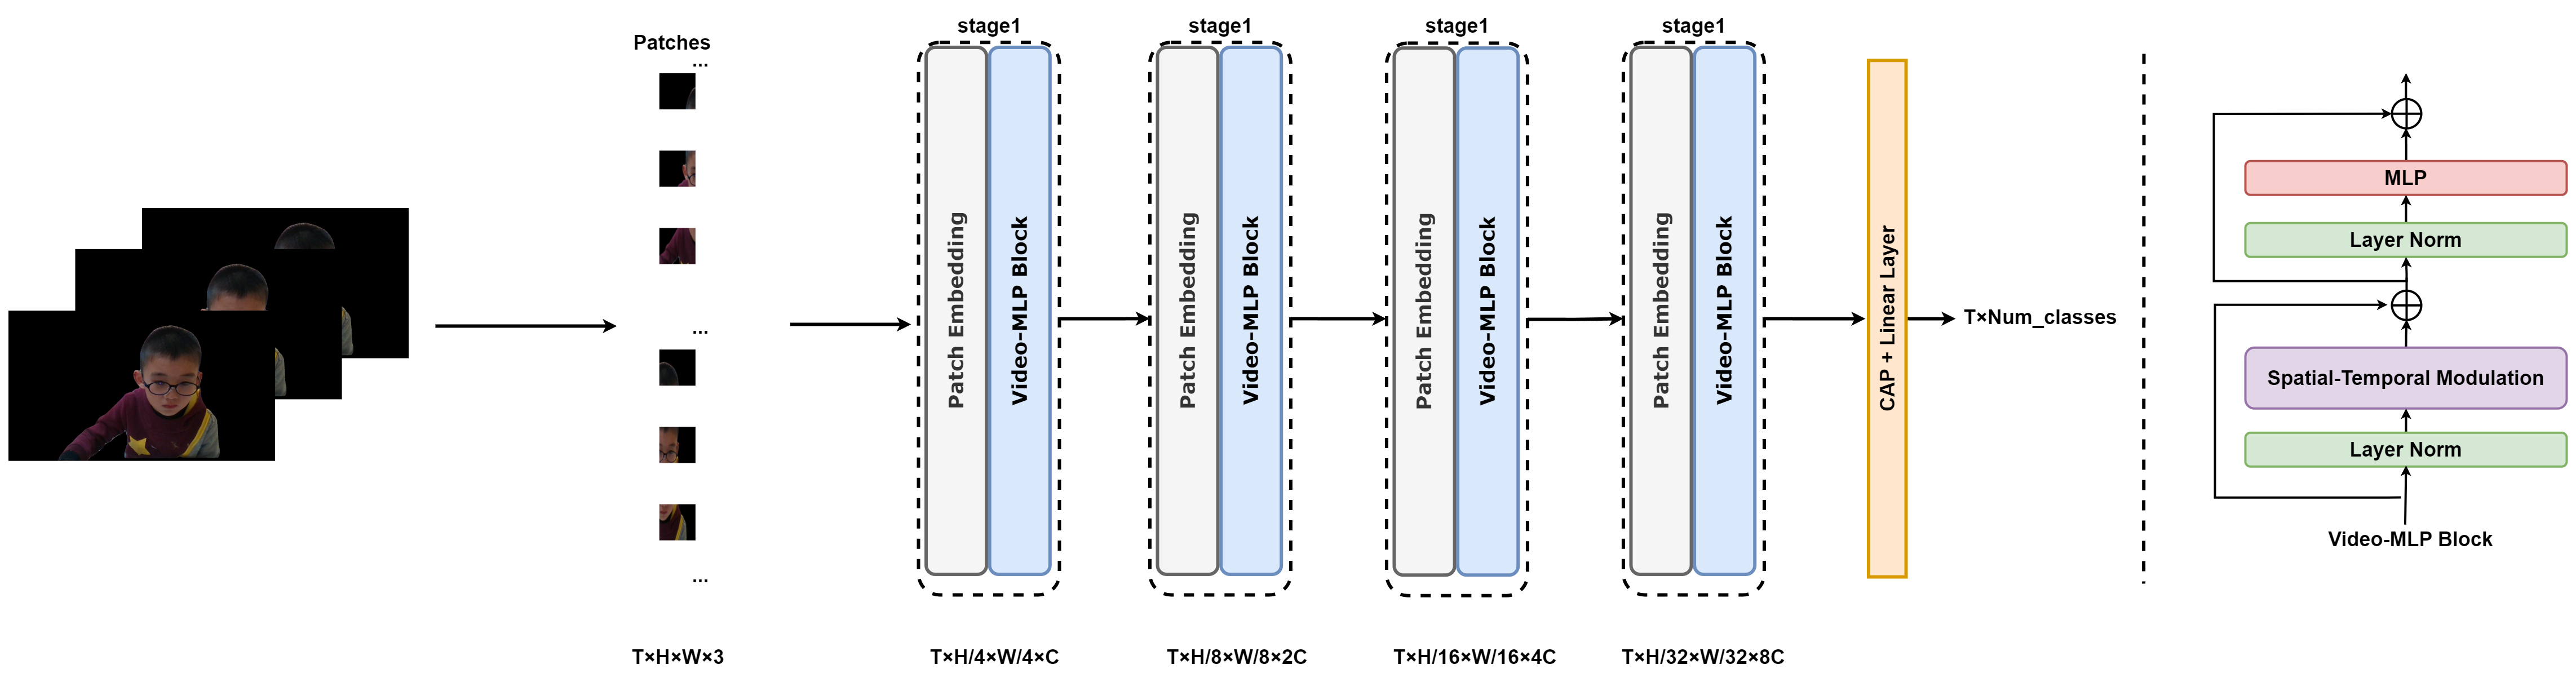
\includegraphics[width=.9\linewidth]{picture/svnet.png}%
  }

\caption{The video modal branch, SVNet, is capable of modeling video data}
\label{fig:two_sub_figures_ieee}
\end{figure*}
\section{PRELIMINARIES}
\label{sec:relatedwork}
\subsection{Self-Attention and Focus Modulation}

Self-attention and focal modulation are two key mechanisms used for modeling spatiotemporal context. 
Self-attention captures spatiotemporal context through interactions between queries and keys,
along with context aggregation. This mechanism is theoretically powerful, 
effectively capturing dependencies between different elements in a sequence. However, 
its computational cost is significant, especially when dealing with large-scale data. 
Each token requires dot product calculations with all other tokens to obtain attention scores,
resulting in a computational complexity of $O(n^2)$.


Unlike self-attention, focal modulation employs a more efficient strategy. 
It first aggregates context and then interacts with the aggregated features through queries. 
This process makes computations more lightweight, reducing computational complexity. 
The design inspiration for focal modulation comes from the concept of adaptive selection. 
The core idea is to selectively perform interactions on the basis of context aggregation, 
thus more effectively capturing key features.

\subsection{Gate Units}
To mitigate the computational complexity of self-attention, spatial gate units (SGUs) are introduced to capture dependencies involving second-order feature interactions (e.g., $z_i \cdot z_j$) across tokens. The input sequence $Z$ for SGU can be represented as $R^{L \times N}$, where $L$ is the length of the input sequence, and $N$ is the token dimension.

SGU can be conceptualized as a combination of two components through element-wise multiplication, expressed as:

\[
s(Z) = [\sigma(ZW_U)] \odot [W_s(\sigma(ZW_V)) + b]   \tag{2}
\]

Here, $W_U$ and $W_V \in \mathbb{R}^{N \times N'}$ represent the weights of the channel projection layer, with the goal of projecting input features into higher-level representations. $W_s \in \mathbb{R}^{L \times L}$ is the weight of the spatial projection layer, fostering communication between any tokens. $b$ is the bias of the spatial projection layer. $\odot$ denotes element-wise multiplication. The right part can be interpreted as an attention map, delineating the significance of each element, as expressed by:

\[
\text{Attention} = W_s(\sigma(ZW_V)) + b   \tag{3}
\]

The values in this context signify the importance of each element. SGU achieves feature selection through element-wise multiplication, with specific weights dynamically parameterized based on the input. This imparts adaptability to SGU not only in the spatial dimension but also in the channel dimension.

In the model, SGU's design attains adaptability in both spatial and channel dimensions, effectively leveraging the advantages of attention mechanisms. This design proficiently captures features with intricate interaction relationships, introducing point-to-point activation to enhance the model's expressive power.
\subsection{Graph Convolution in Action Recognition}
A person's skeleton information can be categorized into key points and bones, where key points function as vertices in the graph, and bones constitute the edges in the graph. Subsequently, based on the set of vertices and edges, the adjacency matrix of the graph can be defined, with the values indicating whether two vertices are connected, forming a sparse matrix.

Graph convolution, specifically referring to channel-weight-shared graph convolution here, involves feature transformation and aggregation operations to derive the feature representation \(Z_j\) of the output node \(v_j\). In this context, \(W\) denotes the weight, \(X_j\) signifies the feature of vertex \(v_j\), and \(a_{ij}\) can be classified into two scenarios. For static methods, \(a_{ij}\) is predefined as learnable parameters. For dynamic methods, \(a_{ij}\) undergoes dynamic transformation based on the input.


Graph convolution, especially in the case of channel-weight-shared graph convolution, involves feature transformation and aggregation operations to derive the feature representation \(Z_j\) of the output node \(v_j\). In this context, \(W\) denotes the weight, \(X_j\) signifies the feature of vertex \(v_j\), and \(a_{ij}\) can be categorized into two scenarios. For static methods, \(a_{ij}\) is predefined as learnable parameters. For dynamic methods, \(a_{ij}\) undergoes dynamic transformation based on the input.


\section{METHODS}
\label{sec:latexhints}

% Required for proper example rendering in the compiled PDF
\newcount\LTGbeginlineexample
\newcount\LTGendlineexample
\newenvironment{ltgexample}%
{\LTGbeginlineexample=\numexpr\inputlineno+1\relax}%
{\LTGendlineexample=\numexpr\inputlineno-1\relax%
%
\tcbinputlisting{%
  listing only,
  listing file=\currfilepath,
  colback=green!5!white,
  colframe=green!25,
  coltitle=black!90,
  coltext=black!90,
  left=8mm,
  title=Corresponding \LaTeX{} code of \texttt{\currfilepath},
  listing options={%
    frame=none,
    language={[LaTeX]TeX},
    escapeinside={},
    firstline=\the\LTGbeginlineexample,
    lastline=\the\LTGendlineexample,
    firstnumber=\the\LTGbeginlineexample,
    basewidth=.5em,
    aboveskip=0mm,
    belowskip=0mm,
    numbers=left,
    xleftmargin=0mm,
    numberstyle=\tiny,
    numbersep=8pt%
  }
}
}%
As shown in the illustration, we use skeleton and RGB-D data as inputs for the entire model. 
Through corresponding branches, the model undergoes forward propagation, 
merging the results from both modalities to obtain the overall output. This model is referred to as SVNet.
 Specifically, SVNet comprises three independent networks: STFNet and CTR-MLP. 
 STFNet processes data from the RGB-D modality, while CTR-MLP handles 2D/3D skeleton data. 
 Through decision fusion, the features generated by these two networks are ultimately combined.More Specifically,
for each of the N training samples in the dataset, we represent the features of the i-th sample as
  \(fJ(i), B(i), V(i)\), where \(J(i)\) is the skeleton joint input, \(B(i)\) is the skeleton bone input,
  and \(V(i)\) is the RGB video input. The corresponding action label is denoted as \(y(i)\). 
  The specific fusion operation is as follows:
\[
\hat{y} = G_J(\theta_J, J) + G_B(\theta_B, B)+ G_V(\theta_V, V) \tag{4}
\]
Next, we will individually introduce the structures of SVNet and DraphMLP, 
concluding with an explanation of our fusion method.



% \subsection{STFNet(Spatio-Temporal Focal Modulation layer)}
% \begin{figure}
%   \centering
%   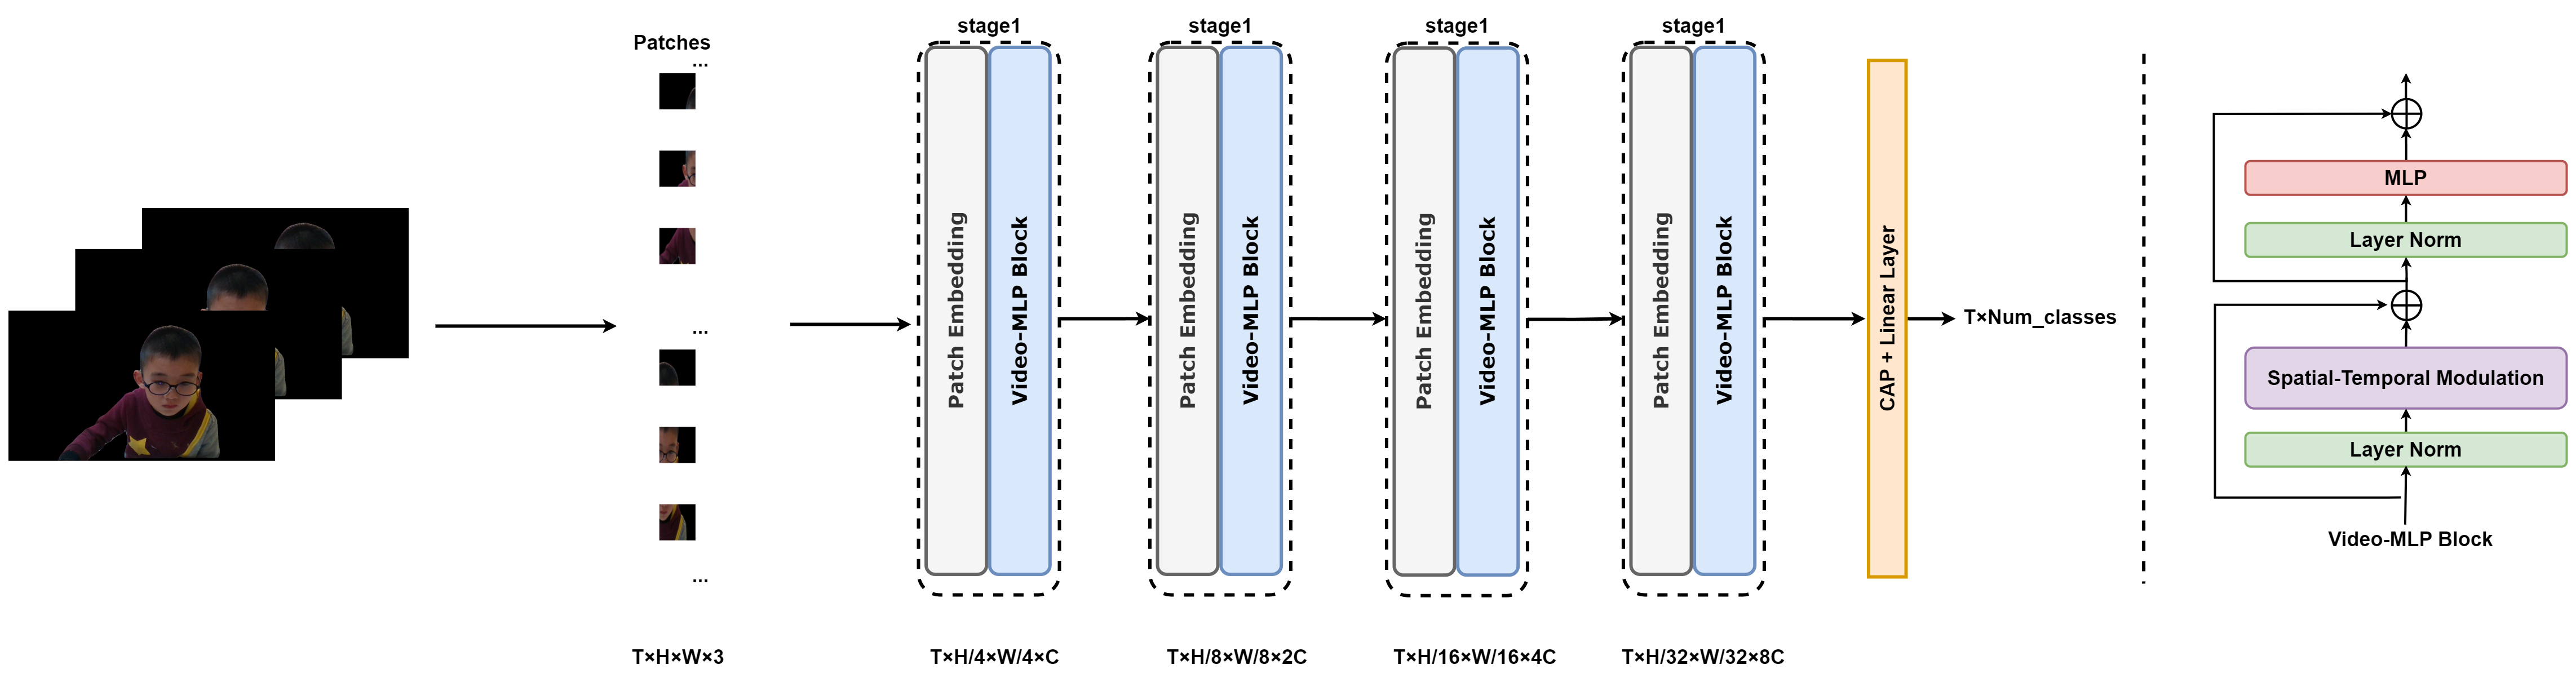
\includegraphics[width=.8\linewidth]{picture/svnet.png}
%   \caption[Simple Figure]{Simple Figure. Based on \citet{mwe}.}
%   \label{fig:label}
% \end{figure}




For the RGB-D modality, our proposed network architecture is based on the VIT network. 
Specifically, we first map tokens to higher dimensions through patch embedding. 
Subsequently, within the video-MLP block, we cleverly integrate these high-dimensional token details 
to ensure effective incorporation of spatial and temporal features. Unlike the VIT network, 
we use spatiotemporal modulation modules in each stage instead of transformers. 
In the final classification stage, we opt for an average pooling 
fully-connected structure to ensure accurate prediction results in the model's output phase.
\subsubsection{Video-MLP Block}

To ease the computational burden of transformer-based models, 
we introduce the "Focal Modulation" mechanism. Unlike self-attention, 
it reduces computations by grouping similar features before interaction. After grouping, 
we still need to consider token relationships. Instead of complex calculations, 
Focal Modulation uses a simple dot product. 
This captures token relationships well while avoiding heavy computations.

For video data, we propose the video-MLP block, designed with two independent branches.
 One focuses on spatial info, the other on temporal. 
 This allows the model to independently yet collaboratively process video data, 
 creating expressive features. 
 The design inherits the benefits of focal modulation while effectively handling short and l
 ong dependencies in videos, optimizing computation and parameters.

\begin{align*}
y_i &= M_1(T_1(x_i, X_{st}), X_{st}) \tag{5}\\
y_i &= T_2(M_2(i, X_{st}), x_i) \tag{6}\\
y_i &= T_{st}(M_s(i_t, X_{st}, t), M_t(i_{hw}, X_{st}, hw), x_i) \tag{7}\\
y_i &= q(x_i) \odot m_s(i_t, X_{st}, t) \odot m_t(i_{hw}, X_{st}, hw) \tag{8}
\end{align*}


\begin{figure*}[!b]
  \centering
  \subfloat[]{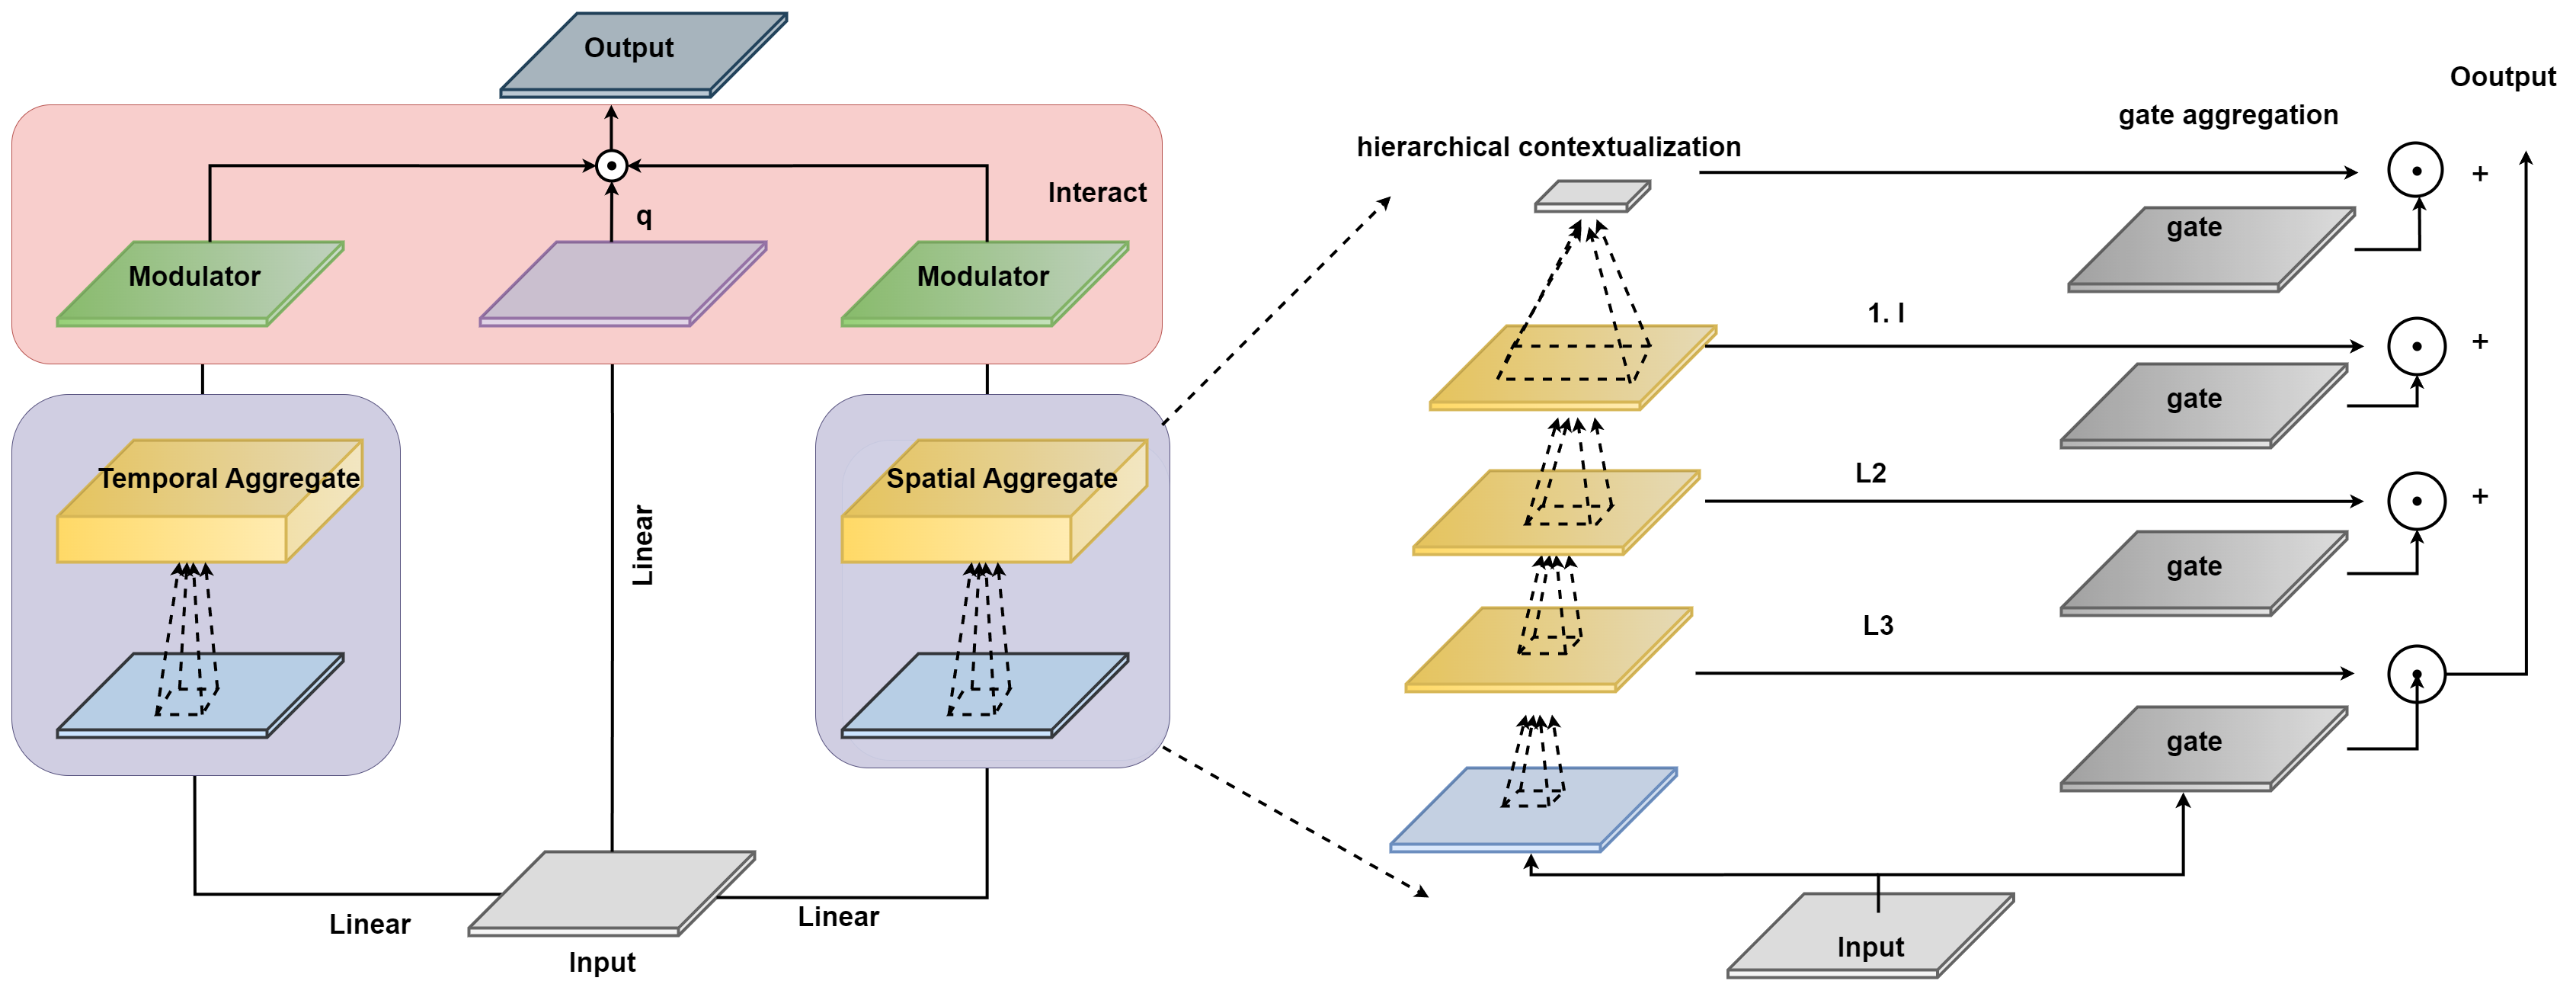
\includegraphics[width=.9\linewidth]{picture/video_mlp_block.png}%
  }

\caption{Focus Modulation and a detailed description of context aggregation in focus modulation}
\label{fig:two_sub_figures_ieee}
\end{figure*}


To model both spatial and temporal contexts for individual tokens,
 it is essential to independently capture spatial and temporal information. Specifically,
  we introduce a dual-stream spatiotemporal local modulation module. Inspired by existing literature, 
  the aggregation process consists of two steps: hierarchical contextualization, 
  extracting context from local to global levels at different granularity levels, 
  and gate aggregation, compressing all contextual features from different granularity levels into 
  modulators. Firstly, linear layers are utilized to project inputs, generating queries, 
  spatial/temporal feature maps, and spatial/temporal gates. Subsequently, through hierarchical
  contextualization \((Ms/Mt)\) and gate aggregation \((Gs/Gt)\), spatial and temporal modulators are created.
  They then interact with query markers through element-wise multiplication, forming the final 
  spatiotemporal feature map.
 Therefore, the spatiotemporal focal modulation process can be defined as follows:
\begin{align*}
  y_i &= q \odot \text{ms}(it, X_{st}, t) \odot \text{mt}(i_{hw}, X_{st}, hw) \tag{9}
  \end{align*}
  Here, \(q(\cdot)\) represents a query projection function, and \(\odot\) denotes 
  element-wise multiplication. \(m_s(\cdot)\) and \(m_t(\cdot)\) are contextual aggregation functions, 
  producing spatial and temporal modulators, respectively. The formulation of \(m_s(\cdot)\) and \(m_t(\cdot)\)
  involves two steps: hierarchical contextualization and gate aggregation.
  



\textbf{Spatio-Temporal Hierarchical Contextualization}

To capture contextual information over short and long distances at different levels of detail, 
the focal modulation mechanism integrates depth-wise convolution. Unlike pooling, depth-wise convolution is 
trainable and structurally aware, operating at the channel level and offering computational efficiency compared 
to regular convolution.

Spatiotemporal depth-wise convolution is applied to the feature map \(X_{st}\), initially mapped through a 
fully connected layer \(f\) to produce the output \(Z = f(Z_{st})\). For computational and parameter efficiency, 
the output \(Z\) undergoes depth-wise convolution operations \(M_{st}\) in both time and space.
 A non-linear transformation using the GeLU activation function follows, and average pooling operations 
 are then applied to the spatial feature map \(Z^s\) and the temporal feature map \(Z^t\). This sequence 
 of steps results in \(L+1\) layers of feature maps, where \(L\) represents the total number of layers in 
 the depth-wise convolution operation.


\begin{align*}
  Z &= f(X_{st})\tag{10} \\
  Z_\ell &= \text{GeLU}(M(Z_{\ell-1}))\tag{11} \\
  Z_{\text{avg}} &= \text{Avg-Pool}(Z)\tag{12}
  \end{align*}
  

% \begin{align*}
%   Z &= f(X_{st}) \\
%   Z_\ell &= \text{GeLU}(M(Z_{\ell-1})) \\
%   Z_{\text{avg}} &= \text{Avg-Pool}(Z) \\
%   Z_0^s &= f_{z,s}(X_{st}) \in \mathbb{R}^{T \times H \times W \times C}, \\
%   Z_0^t &= f_{z,t}(X_{st}) \in \mathbb{R}^{T \times H \times W \times C}, \\
%   Z_{\ell}^s &= f_{\ell,a,s}(Z_{\ell-1}^s) \triangleq \text{GeLU}(\text{MLP}(Z_{\ell-1}^s)) \in \mathbb{R}^{T \times H \times W \times C}, \\
%   Z_{\ell}^t &= f_{\ell,a,t}(Z_{\ell-1}^t) \triangleq \text{GeLU}(\text{MLP}(Z_{\ell-1}^t)) \in \mathbb{R}^{T \times H \times W \times C}, \\
%   Z_{L+1}^s &= \text{Avg-Pool}(Z_L^s), \\
%   Z_{L+1}^t &= \text{Avg-Pool}(Z_L^t).
%   \end{align*}
  


\textbf{Spatio-Temporal Gated Aggregation}

To effectively capture and integrate spatiotemporal features in video data, 
we condense the (L + 1) feature maps obtained from hierarchical contextualization into a modulator. 
In images, the relationship between a visual token (query) and its surrounding context often depends on the content itself.
 For instance, the model may rely on local fine-grained features to encode queries about visually salient 
 objects but primarily use global coarse-grained features to encode queries about the background scene.
Based on this intuition, we use a gating mechanism to control the amount of aggregation for each query from
different hierarchical levels. Specifically, for each feature layer, we extract linear weights, 
such as \(G_s\) and \(G_t\), from the spatiotemporal feature map \(X_{st}\). Through these gating weights,
we adjust the output of each feature layer using dot-product operations. 
This means that the output of each feature layer is modulated by its gating weight. 
Finally, these weighted feature maps are aggregated into a single output containing spatiotemporal features 
adjusted and aggregated through gating.

\[
G = G \odot Z\tag{13}
\]
\begin{align*}
  Z_{\text{out}^s} &= \sum_{\ell=1}^{L+1} G_{\ell}^s \odot Z_{\ell}^s \in \mathbb{R}^{H \times W \times C}\tag{14} \\
  Z_{\text{out}^t} &= \sum_{\ell=1}^{L+1} G_{\ell}^t \odot Z_{\ell}^t \in \mathbb{R}^{T \times C}\tag{15}
\end{align*}

Where$(\odot)$ denotes the dot-product operation. \(Z_{\text{out}}\) is the output of aggregated and gated spatiotemporal features.
To facilitate communication across different channels, another set of linear layers, \(h_s(\cdot)\) and \(h_t(\cdot)\), are used to obtain the spatial modulator (\(M_s = h_s(Z_{\text{out}_s}) \in \mathbb{R}^{T \times H \times W \times C}\)) and the temporal modulator (\(M_t = h_t(Z_{\text{out}_t}) \in \mathbb{R}^{T \times H \times W \times C}\)), respectively. Therefore, the spatiotemporal focal modulation process defined by the equation can be rewritten as:
\[ y_i = q(x_i) \odot h_s\left(\sum_{l=1}^{L+1} g_{li,s} \odot z_{li,s}\right) \odot h_t\left(\sum_{l=1}^{L+1} g_{li,t} \odot z_{li,t}\right) \quad (16) \]





\subsection{GraphMLP}
\begin{figure}
  \centering
  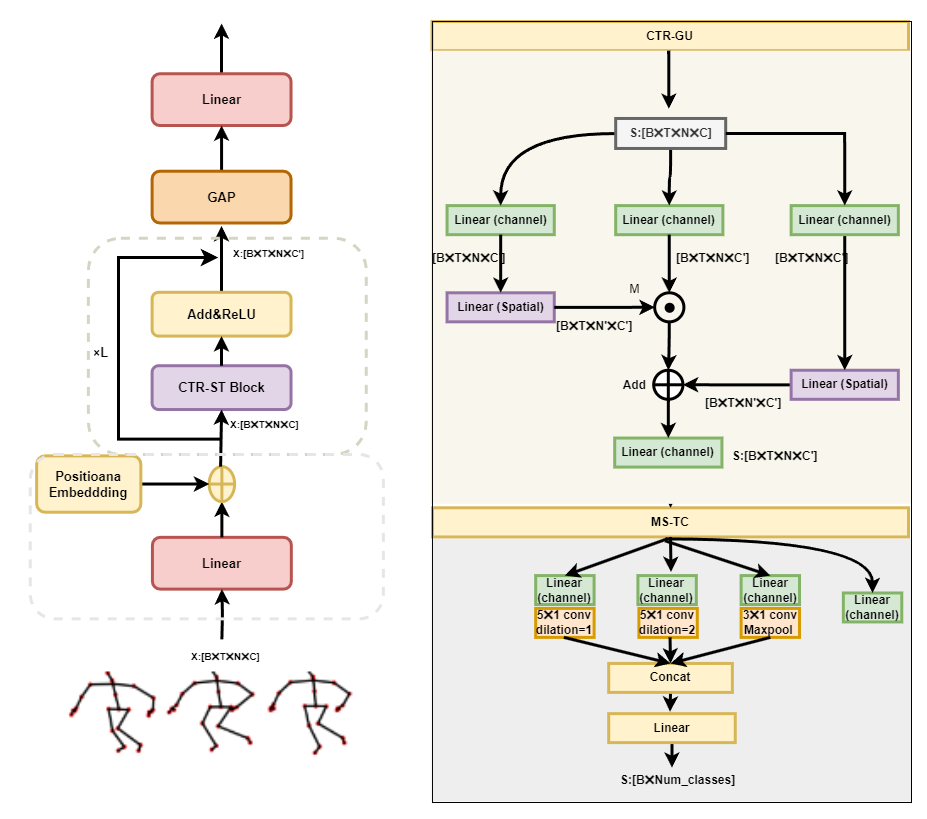
\includegraphics[width=.8\linewidth]{picture/CTR-MLP.png}
  \caption[Simple Figure]{Skeletal branches:Model architecture overview and description. Embedding blocks are used to preserve location information. The CTR\-STGU module captures spatial dependencies, and the MS-TC module aggregates temporal information. The global average pooling layer is used to aggregate the global spatiotemporal union information of the final linear classifier..}
  \label{fig:label}
\end{figure}

In this section, we introduce a straightforward neural network architecture named CTR-MLP, 
designed for skeleton-based human action recognition. The entire network consists of an embedding block, 
5 basic blocks, and a global average pooling layer, followed by a linear classifier for action category 
prediction. To address the complexity of joint spatiotemporal optimization, 
drawing inspiration from previous works like CTR-GCN, we embed spatial STGU and temporal MS-TC modules 
in a sequential manner within the basic blocks. Specifically, CTR-MLP is formed by stacking these basic
 modules, with the global average pooling layer efficiently aggregating spatiotemporal information for 
 the final linear classifier input. Despite some convolutional operations in the temporal modeling module,
 CTR-MLP is primarily composed of linear layers.

\subsubsection{Spatial Modeling}
Motivated by the CTR-GC module in CTR-GCN, we developed the CTR-GC module featuring a gating mechanism. 
In contrast to prior approaches, this method adopts a single branch dedicated to spatial information 
extraction without making any predefined assumptions. In comparison, the typical CTR-GC module necessitates 
three parallel branches to integrate various human priors. The gating mechanism, employing element-wise
multiplication, empowers the network to smartly select and focus on the most discriminative features
guided by the generated attention maps. 
This design enhances the network's adaptability, enabling it to efficiently choose crucial features.

\begin{algorithm}
  \renewcommand{\algorithmicrequire}{\textbf{Input:}}
  \renewcommand{\algorithmicensure}{\textbf{Output:}}
  \caption{STGU Algorithm}
  \label{alg:stgu}
  \begin{algorithmic}[1]
    \REQUIRE Input tensor $x$ of shape $(B, T, V, C)$, out-channel $d_{\text{model}}$, number of joints $num_{\text{joints}}$
    \ENSURE Output tensor of shape $(B, T, V, C)$
    \STATE $shortcut \leftarrow x$
    \STATE $x \leftarrow \text{norm}(x, \text{axis}="channel")$
    \STATE $x \leftarrow \text{proj}(x, 3 \times d_{\text{model}}, \text{axis}="channel")$
    \STATE $F_1, F_2, F_3 \leftarrow \text{split}(x, \text{axis}="channel")$
    \STATE $M \leftarrow \text{proj}(F_2, num_{\text{joints}}, \text{axis}="spatial", \text{init\_weight}=0)$
    \STATE $F_p \leftarrow F_1 \times M$
    \STATE $F_s \leftarrow \text{proj}(F_3, num_{\text{joints}}, \text{axis}="spatial")$
    \STATE $H \leftarrow \text{proj}((F_s + F_p), d_{\text{model}}, \text{axis}="channel")$
    \RETURN $shortcut + H$
  \end{algorithmic}  
\end{algorithm}

Specifically, we start by applying channel normalization to the input tensor, 
ensuring data stability and consistency. Next, by expanding the feature dimension, 
we provide more information space for subsequent operations. In particular, the original feature tensor 
is divided into three distinct parts, allowing the capture and representation of different levels of 
spatial patterns and structures. The 'M' part employs an attention mechanism, applying weight adjustments 
to one of the feature parts, enabling the model to focus more on certain key information when processing 
spatiotemporal data. This attention mechanism helps capture and reinforce spatial patterns relevant to 
the input data, thereby enhancing the model's performance. Finally, the processed features are combined 
with the original input, ensuring that key information from the original data is not lost during feature 
enhancement, while also obtaining a richer and more detailed feature representation. This design 
aims to provide a more powerful and effective data representation for subsequent spatiotemporal tasks.



\subsubsection{Temporal Modeling}
We employ four parallel branches, each utilizing different kernel sizes \(k_i\), 
dilation rates \(d_i\), and max-pooling operations to capture multiscale temporal information. 
The features extracted from these branches are concatenated to form a feature representation 
that integrates multiscale temporal information. The MS-TC operation can be expressed as follows:

\begin{align*}
  Y(l) = \text{MS-TC}(H(l)) = \text{Concat}(\text{Conv}_{k_i, d_i}(H(l)))\tag{17} , \\i = 1,2,3,4
\end{align*}
 
  Here, \(l\) is the index of stacked basic blocks, \(H(l)\) represents the features 
  processed by STGU, \(\text{Conv}_{k_i, d_i}(\cdot)\) denotes the convolution operation, 
  and \(\text{Concat}(\cdot)\) signifies the concatenation operation.The CTR-MLP model is constructed by iteratively stacking STGU and MS-TC modules, 
  where each basic block performs spatiotemporal modeling through STGU and then conducts 
  multiscale temporal convolution via MS-TC. The residual connections ensure stable gradient 
  propagation and smooth training, while the introduction of ReLU activation layers enhances 
  the model's non-linear expressive capacity. The overall temporal modeling process, 
  achieved through stacking basic blocks, aims to comprehensively capture the rich features 
  of actions in both time and space. The construction process for a basic block in CTR-MLP 
  can be expressed as follows:
  
\begin{align*}
  H(l) &= \text{STGU}(X(l))\tag{18} \\
  X(l+1) &= \text{ReLU}(Y(l) + X(l))\tag{19}
  \end{align*}
  Here, \(l\) represents the index of stacked basic blocks, \(X(l)\) denotes the input features, and \(Y(l)\) signifies the features processed by MS-TC.
  



\begin{figure*}[!b]
  \centering
  \subfloat[]{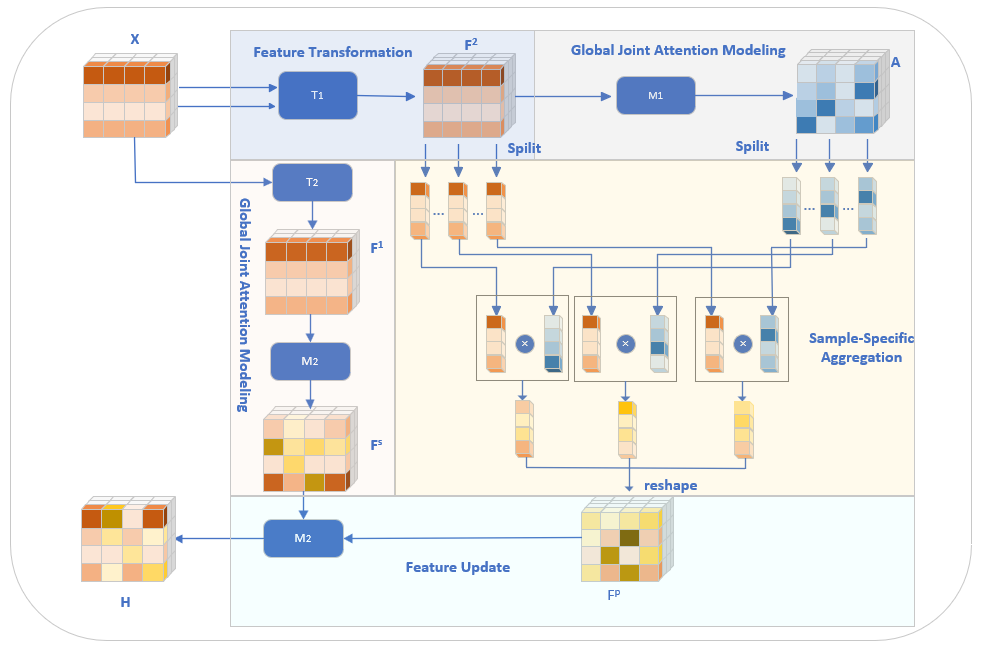
\includegraphics[width=.9\linewidth]{picture/Graph_MLP.png}%
  }

\caption{The framework of the proposed spatial topological gate elements. Feature transformation, which aims to transform the input features into the potential high dimensional feature space, model the global joint attention, and construct the entire independent topological attention. sample specific aggregation, which aims to select dynamic features for the current sample; Trait updates, which aim to fuse and update aggregated features}

\end{figure*}



Our STGU has a four-part framework, shown in the figure. It includes four parts: (1) Feature Transformation,
 aiming to transform input features into a potential high-dimensional feature space; 
 (2) Global Joint Attention Modeling, constructing independent topological attention across 
 the entire structure; (3) Sample-Specific Aggregation, designed to select dynamic features for 
 the current sample; (4) Feature Update, focused on merging and updating the aggregated features. 
 The Channel Linear Layer \(T(\cdot)\) works on feature channels, merging spatial features across 
 different channels. The Spatial Linear Layer \(M(\cdot)\) operates on joint features, capturing 
 spatial information independently for all joints across each channel and frame. Let's delve into each block.

1. \textbf{Feature Transformation:} The model undergoes the Feature Transformation stage, 
denoted as \(T_i\) in the diagram, which maps the input spatiotemporal features to a higher-dimensional 
feature space. The crucial aspect of this step is the temporal linear transformation, 
achieved through the weight matrix \(W_i\), transforming the input features \(X\) into a new feature 
representation \(F_i\). This process enriches the feature representation for subsequent attention mechanisms.
   \[
   F_i = \sigma(XW_i),i=1,2 \tag{20}
   \]

2. \textbf{Global Joint Attention Modeling:} We apply the same operation used in feature transformation 
to project the input into a latent feature space. Subsequently, we employ a spatial linear layer to 
facilitate communication across joints, denoted as \(M_1\). 
This inter-joint communication provides a global receptive field for the attention map of the current pose.
 The importance of each node is dynamically adjusted through spatial linear layers and dynamic 
 parameters \(W_A/W_s\). Specifically:
   \[
    A = W_A(\sigma(F_2)), \quad F_s = W_SF_1\tag{21}
   \]

3. \textbf{Sample-Specific Aggregation:} Sample-Specific Aggregation:
 By transforming features \(F_1\) and the defined attention map \(A\), 
 we split them along the channel and temporal dimensions. This implies that the spatiotemporal 
 topological features and spatiotemporal attention can be viewed as sets of vectors, perfectly 
 aligned in both channel and temporal dimensions. Each topological vector corresponds to an attention 
 vector. We employ element-wise multiplication in gating units, allowing the network to selectively focus 
 on features of interest based on the generated attention map. 
This aggregation method captures intricate spatial interactions across joints.
   \[
   F_p = F_1 \odot A\tag{22}
   \]

   This point-wise aggregation effectively captures dynamic temporal attention and preserves topological 
   attention across channels. 
   It can be computed in parallel with minimal computational overhead.



4. \textbf{Feature Update:} In the final stage of feature updating, the model blends the sample-specific 
aggregated feature \(F_p\) and Global Joint Attention feature \(F_s\). This fusion is achieved through 
a projection layer, producing the ultimate output tensor \(H\). This tensor encapsulates the comprehensive 
modeling of intricate spatiotemporal relationships in the input data. The crucial 
aspect here is striking a balance between individual sample specificity and overall sample commonality.
   \[
   H = \sigma(F_p + F_s)W_O\tag{23}
   \]

   STGU, with smart attention mechanisms and pointwise aggregation, 
   ensures early-stage behavior resembling a conventional GCN. \(W_S\), A, and \(W_O\) matrices play 
   key roles. This initialization proves crucial for model convergence. Over ongoing training, 
   STGU progressively incorporates sample-specific 
   spatial information, effectively capturing intricate spatiotemporal relationships.




    \begin{figure*}[!b]
        \centering
        \subfloat[]{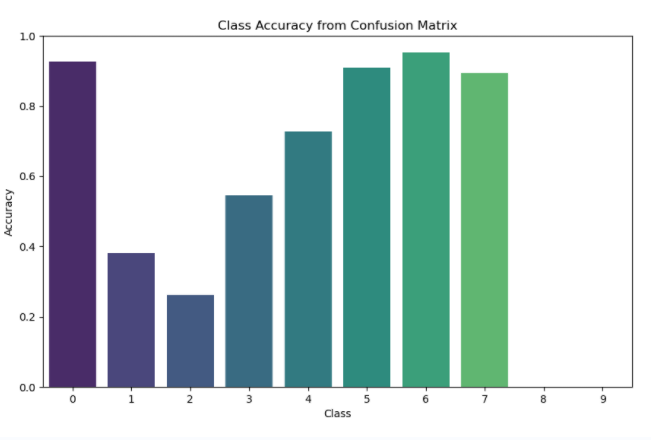
\includegraphics[width=.3\linewidth]{picture/joint.png}%
        \label{fig:first_case_ieee}}
      \hfil
        \subfloat[]{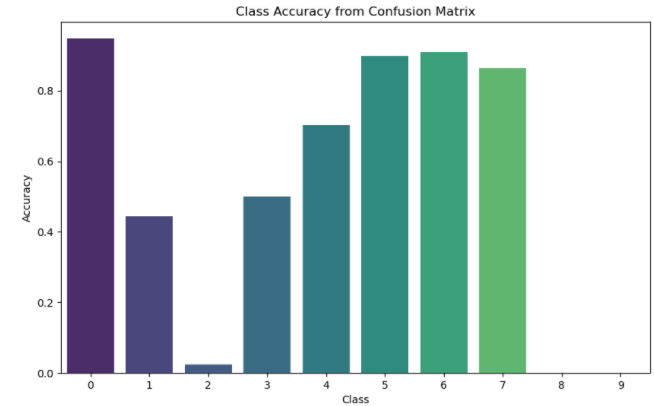
\includegraphics[width=.3\linewidth]{picture/bone.png}%
        \label{fig:second_case_ieee}}
      \hfil
        \subfloat[]{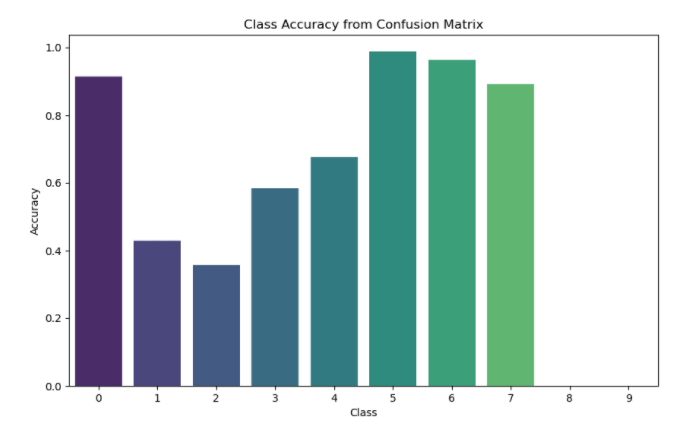
\includegraphics[width=.3\linewidth]{picture/fuse.png}%
        \label{fig:second_case_ieee}}
      \caption{The accuracy of each type of ADHD}
      \label{fig:two_sub_figures_ieee}
    \end{figure*}

    




    \begin{figure*}[!b]
        \centering
        \subfloat[]{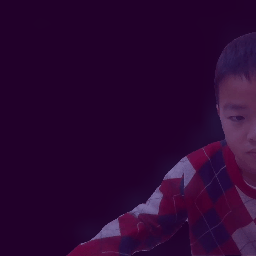
\includegraphics[width=.15\linewidth]{gif/1/frame_001.png}%
        \label{fig:first_case_ieee}}
      \hfil
        \subfloat[]{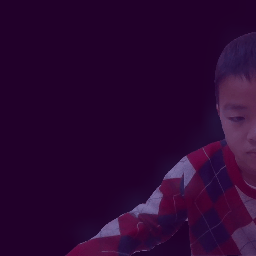
\includegraphics[width=.15\linewidth]{gif/1/frame_009.png}%
        \label{fig:second_case_ieee}}
      \hfil
        \subfloat[]{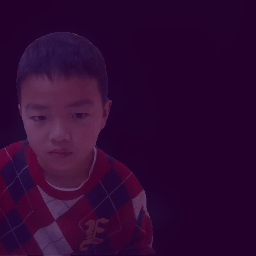
\includegraphics[width=.15\linewidth]{gif/1/frame_017.png}%
        \label{fig:second_case_ieee}}
      \hfil
        \subfloat[]{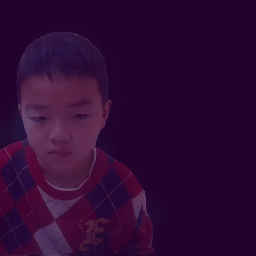
\includegraphics[width=.15\linewidth]{gif/1/frame_025.png}%
        \label{fig:second_case_ieee}}
      \hfil
      \subfloat[]{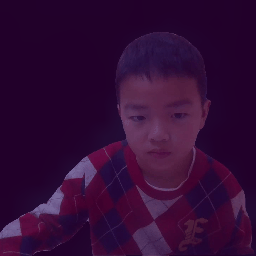
\includegraphics[width=.15\linewidth]{gif/1/frame_033.png}%
        \label{fig:second_case_ieee}}
      \hfil
        \subfloat[]{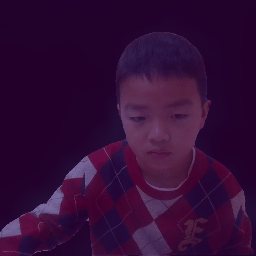
\includegraphics[width=.15\linewidth]{gif/1/frame_041.png}%
        \label{fig:second_case_ieee}}
      \hfil
        \subfloat[]{
\includegraphics[width=.15\linewidth]{gif/2/frame_001.png}%
        \label{fig:first_case_ieee}}
      \hfil
        \subfloat[]{
\includegraphics[width=.15\linewidth]{gif/2/frame_009.png}%
        \label{fig:second_case_ieee}}
      \hfil
        \subfloat[]{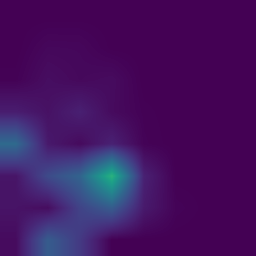
\includegraphics[width=.15\linewidth]{gif/2/frame_017.png}%
        \label{fig:second_case_ieee}}
      \hfil
        \subfloat[]{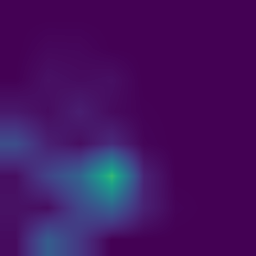
\includegraphics[width=.15\linewidth]{gif/2/frame_025.png}%
        \label{fig:second_case_ieee}}
      \hfil
      \subfloat[]{
\includegraphics[width=.15\linewidth]{gif/2/frame_033.png}%
        \label{fig:second_case_ieee}}
      \hfil
        \subfloat[]{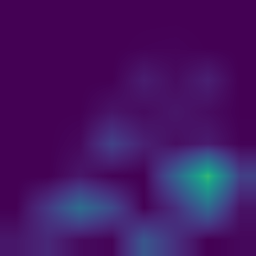
\includegraphics[width=.15\linewidth]{gif/2/frame_041.png}%
        \label{fig:second_case_ieee}}
  
      \caption{SFTNet visualization}
      \label{fig:two_sub_figures_ieee}
    \end{figure*}


    
    
    

    

\section{Results and Analysis}




\subsection{Experimental Setup and Protocols}




\subsection{Comparison with State-of-the-art}
\textbf{Kinetics-400:} On the K400 dataset, we present the results of SFTNet and compare them with classical methods in the table. 
Despite a slight decrease of about one percentage point compared to the latest Swin-B/S/T models, 
our approach significantly reduces TFLOPs by over 50\%, even surpassing Swin-T. 
Our model not only outperforms most classical models in accuracy but also achieves remarkably low TFLOPs.

\begin{table}[ht]
  \centering
  \caption{Comparison with state-of-the-art methods on Kinetics\-400 dataset.}
  \resizebox{250pt}{!}{
  \begin{tabular}{|l|l|l|l|l|}
  \hline
  \textbf{Model} & \textbf{Pre-training} & \textbf{Top-1} & \textbf{FLOPs (G)} & \textbf{Params (M)} \\
  \hline
  TSN & ImageNet & 73.8 & 102.76 & 24.33 \\
  TSM & ImageNet & 73.18 & 32.88 & 23.87 \\
  I3D & ImageNet & 74.8 & 59.30 & 35.40 \\
  R2plus1D & - & 75.46 & 13.00 & 63.80 \\
  SlowFast & - & 75.55 & 36.30 & 34.50 \\
  TaNet & ImageNet & 76.25 & 43.00 & 25.60 \\
  TimesFormer (divst) & ImageNet-21K & 77.69 & 196.00 & 122.00 \\
  CSN & IG65M & 82.87 & 67.63 & 29.70 \\
  MVIT & - & 80.60 & 64.00 & 34.50 \\
  Video-Swin-T & ImageNet-1K & 78.9 & 88.00 & 28.20 \\
  Video-Swin-S & ImageNet-1K & 80.54 & 166.00 & 49.80 \\
  Video-Swin-B & ImageNet-1K & 80.57 & 282.0. & 88.0 \\
  \textbf{SFTNet} & \textbf{ImageNet-1K} & \textbf{79.6} & \textbf{63} & \textbf{19.45} \\
  \hline
  \end{tabular}
  }
  \label{tab:model_comparison}
  \end{table}


\textbf{NTU60\_Xsub\_2D: }Compared to existing models, our approach maintains competitiveness in accuracy,
 with a difference of only two to three percentage points from the optimal model. While slightly 
 trailing behind the MSG3D and PoseC3D models in this aspect, our model exhibits distinct advantages 
 in other areas. From the perspective of FLOPs and Params, our model demonstrates outstanding efficiency.
  Compared to the MSG3D model, FLOPs decrease by approximately 70\%, while Params decrease by nearly 14 
  times. This implies that our model efficiently utilizes computational resources while providing comparable 
  accuracy. Despite a slight accuracy reduction compared to certain models, considering the significant 
  decrease in FLOPs and Params, our model still holds advantages in practical applications. 
  This indicates that our model has achieved a good balance between performance and efficiency.

  \begin{table}[h]
    \centering
    \caption{Comparison with state-of-the-art methods on NTU60\_Xsub\_2D dataset.}
    \label{tab:model_comparison}
    \resizebox{250pt}{!}{
    \begin{tabular}{|l|l|c|c|c|}
    \hline
    \textbf{Model} & \textbf{Modality} & \textbf{Top-1} & \textbf{FLOPs} & \textbf{Params} \\
    \hline
    2s-agcn & joint & 88.60 & 4.40 & 3.50 \\
            & bone  & 91.59 & 4.40 & 3.50 \\
    STGCN   & joint & 88.95 & 3.80 & 3.10 \\
            & bone  & 91.69 & 3.80 & 3.10 \\
    STGCNPP & joint & 89.26 & 1.95 & 1.39 \\
            & bone  & 92.30 & 1.95 & 1.39 \\
    MSG3D   & joint & 92.3  & 37.09 & 14.28 \\
            & bone  &       &       &       \\
    PoseC3D  & joint & 93.60 & 20.60 & 2.00 \\
            & bone  & 93.50 & 20.60 & 2.00 \\
    CTRGCN  & joint & 89.6  & 8.142 & 1.95 \\
            & bone  & -     & 8.142 & 1.95 \\
    \textbf{CTRMLP} & \textbf{joint} & \textbf{89.2} & \textbf{6.58} & \textbf{2.64} \\
                  & \textbf{bone}  &       & \textbf{6.58} & \textbf{2.64} \\
    \hline
    \end{tabular}
    }
    \end{table}
    
\textbf{ADHD Data: }Our proposed model demonstrates significant performance advantages
 on the self-collected dataset. Compared to recent SOTA models, our model achieves an 
 improvement of nearly 3 percentage points in accuracy, surpassing the Xclip model and 
 slightly outperforming the Video\_Swin model. Moreover, 
our model achieves a smaller scale in terms of computational complexity and parameter count.

\begin{table}[ht]
  \centering
  \caption{SVnet test results on the ADHD dataset}
  \resizebox{250pt}{!}{
  \begin{tabular}{|c|c|c|c|c|c|}
  \hline
  \textbf{Modality} & \textbf{Method} & \textbf{Accuracy} & \textbf{Flops} & \textbf{Params} & \textbf{Fusion} \\
  \hline
  RGB-Video & Video\_swin & 0.8749 & 0.543T & 87.649M & 0.8817 \\
  RGB-Video & Timesformer & 0.7082 & 0.196T & 0.121G & \\
  RGB-Video & SlowFast & 0.8306 & 94.827G & 34.566M & \\
  RGB-Video & Xclip & \textbf{0.8564} & -- & -- & \\
  RGB-Video & \textbf{SFTNet} & \textbf{0.8836} & 63.112G & 49.553M & \\
  \hline
  \end{tabular}
  }
  \end{table}

  \begin{table}[ht]
    \centering
    \caption{Graph\-MLP test results on the ADHD dataset}
    \resizebox{250pt}{!}{
    \begin{tabular}{|c|c|c|c|c|}
    \hline
    \textbf{Modality} & \textbf{Method} & \textbf{Joint} & \textbf{Bone} & \textbf{Fusion} \\
    \hline
    Skeleton-2D & STGCN & 0.8115 & 0.7792 & 0.8147 \\
                & 2SGCN & 0.8325 & 0.8084 & 0.8414 \\
                & MSGCN & 0.8428 & 0.8376 & 0.8452 \\
                & STGCNPP & 0.8147 & 0.8211 & 0.8388 \\
                & CTRGCN & 0.8426 & 0.8293 & 0.8471 \\
                & POSEC3D & 0.8106 & 0.7925 & 0.8258 \\
                & \textbf{CTRMLP} & \textbf{0.8408} & \textbf{0.8258} & \textbf{0.8457} \\
    Skeleton-3D & CTRGCN-3D & 0.7226 & 0.6600 & 0.7248 \\
                & STGCNPP-3D & 0.6644 & 0.7231 & 0.7383 \\
                & 2SGCN-3D & 0.7091 & 0.6980 & 0.7092 \\
    \hline
    \end{tabular}
    }
    \end{table}
    
  

\subsection{ Ablations}

\subsubsection{The structure of the modulator}

\begin{table}[ht]
  \centering
  \caption{Comparison of Different Models}
  \resizebox{250pt}{!}{
  \begin{tabular}{|c|c|c|}
  \hline
  \textbf{FocalModule} & \textbf{Accuracy} & \textbf{Params} \\
  \hline
  Parallel & 0.8836 & 49.553M \\
  Serial1 & 0.8675 & 156.989M \\
  Serial2 & 0.8052 & 156.989M \\
  \hline
  \end{tabular}
  }
  \end{table}
  
  \subsubsection{Spatiotemporal interaction methods}
  \subsubsection{Validity of the STGU component}
  \subsubsection{Convergence of decisions}






\section{CONCLUSION}

% 在某个位置开始新页面
\newpage
\newpage
\subsection{Cleveref examples}
\label{sec:ex:cref}

Cleveref demonstration: Cref at beginning of sentence, cref in all other cases.


\begin{ltgexample}
\Cref{fig:ex:cref} shows a simple fact, although \cref{fig:ex:cref} could also show something else.

\Cref{tab:ex:cref} shows a simple fact, although \cref{tab:ex:cref} could also show something else.

\Cref{sec:ex:cref} shows a simple fact, although \cref{sec:ex:cref} could also show something else.
\end{ltgexample}

\subsection{Figures}

\begin{ltgexample}
\Cref{fig:label} shows something interesting.

\begin{figure}
  \centering
  \includegraphics[width=.8\linewidth]{example-image-golden}
  \caption[Simple Figure]{Simple Figure. Based on \citet{mwe}.}
  \label{fig:label}
\end{figure}
\end{ltgexample}

One can span a figure across multiple columns by using \verb+\begin{figure*}+.
See \cref{fig:16x9} as an example.

\begin{ltgexample}
\begin{figure*}
  \centering
  % note that \textwidth is used instead of \linewidth
  % This ensures that the graphics width is 60% of the "page" (text block), and not just 60% of the current text column
  % See https://tex.stackexchange.com/a/17085/9075 for details
  \includegraphics[width=.6\textwidth]{example-image-16x9}
  \caption{16x9 Figure}
  \label{fig:16x9}
\end{figure*}
\end{ltgexample}


\subsection{Sub Figures}

An example of two sub figures is shown in \cref{fig:two_sub_figures}.



Note that often IEEE papers with subfigures do not employ subfigure
captions (using the optional argument to \verb+\subfloat[]+), but instead will
reference/describe all of them (a), (b), etc., within the main caption.
Be aware that for subfig.sty to generate the (a), (b), etc., subfigure
labels, the optional argument to \verb+\subfloat+ must be present. If a
subcaption is not desired, just leave its contents blank,
e.g., \verb+\subfloat[]+.
An example is shown in \cref{fig:two_sub_figures_ieee}.


\subsection{Tables}

Note that IEEE does not support \verb+\begin{table}+, one has to use \verb+\begin{figure}+.

\begin{ltgexample}
\begin{figure}
  \caption{Simple Table}
  \label{tab:simple}
  \centering
  \begin{tabular}{ll}
    \toprule
    Heading1 & Heading2 \\
    \midrule
    One      & Two      \\
    Thee     & Four     \\
    \bottomrule
  \end{tabular}
\end{figure}
\end{ltgexample}

\begin{ltgexample}
% Source: https://tex.stackexchange.com/a/468994/9075
\begin{figure}
\caption{Table with diagonal line}
\label{tab:diag}
\begin{center}
\begin{tabular}{|l|c|c|}
\hline
\diagbox[width=10em]{Diag\\Column Head I}{Diag Column\\Head II} & Second & Third \\
\hline
& foo & bar \\
\hline
\end{tabular}
\end{center}
\end{figure}
\end{ltgexample}


\subsection{Source Code}

\begin{ltgexample}
\Cref{lst:XML} shows source code written in XML.
\Cref{line:comment} contains a comment.

\begin{lstlisting}[
  language=XML,
  caption={Example XML Listing},
  label={lst:XML}]
<listing name="example">
  <!-- comment --> (* \label{line:comment} *)
  <content>not interesting</content>
</listing>
\end{lstlisting}
\end{ltgexample}

One can also add \verb+float+ as parameter to have the listing floating.
\Cref{lst:flXML} shows the floating listing.

\begin{ltgexample}
\begin{lstlisting}[
  % one can adjust spacing here if required
  % aboveskip=2.5\baselineskip,
  % belowskip=-.8\baselineskip,
  float,
  language=XML,
  caption={Example XML listing -- placed as floating figure},
  label={lst:flXML}]
<listing name="example">
  Floating
</listing>
\end{lstlisting}
\end{ltgexample}

One can also typeset JSON as shown in \cref{lst:json}.

\begin{ltgexample}
\begin{lstlisting}[
  float,
  language=json,
  caption={Example JSON listing -- placed as floating figure},
  label={lst:json}]
{
  key: "value"
}
\end{lstlisting}
\end{ltgexample}

Java is also possible as shown in \cref{lst:java}.

\begin{ltgexample}
\begin{lstlisting}[
  caption={Example Java listing},
  label=lst:java,
  language=Java,
  float]
public class Hello {
    public static void main (String[] args) {
        System.out.println("Hello World!");
    }
}
\end{lstlisting}
\end{ltgexample}

\subsection{Itemization}

One can list items as follows:

\begin{ltgexample}
\begin{itemize}
\item Item One
\item Item Two
\end{itemize}
\end{ltgexample}

With the package paralist, one can create itemizations with lesser spacing:

\begin{ltgexample}
\begin{compactitem}
\item Item One
\item Item Two
\end{compactitem}
\end{ltgexample}

One can enumerate items as follows:

\begin{ltgexample}
\begin{enumerate}
  \item Item One
  \item Item Two
\end{enumerate}
\end{ltgexample}

With the package paralist, one can create enumerations with lesser spacing:

\begin{ltgexample}
\begin{compactenum}
  \item Item One
  \item Item Two
\end{compactenum}
\end{ltgexample}

With paralist, one can even have all items typset after each other and have them clean in the tex document:

\begin{ltgexample}
\begin{inparaenum}
  \item All these items...
  \item ...appear in one line
  \item This is enabled by the paralist package.
\end{inparaenum}
\end{ltgexample}

\subsection{Other Features}

\begin{ltgexample}
The words \enquote{workflow} and \enquote{dwarflike} can be copied from the PDF and pasted to a text file.
\end{ltgexample}

\begin{ltgexample}
The symbol for powerset is now correct: $\powerset$ and not a Weierstrass p ($\wp$).

$\powerset({1,2,3})$
\end{ltgexample}

\begin{ltgexample}
Brackets work as designed:
<test>
One can also input backquotes in verbatim text: \verb|`test`|.
\end{ltgexample}


\section{Conclusion and Outlook}
\label{sec:outlook}
\lipsum[1-2]

% regular IEEE prefers the singular form
\section*{Acknowledgment}

Identification of funding sources and other support, and thanks to individuals and groups that assisted in the research and the preparation of the work should be included in an acknowledgment section, which is placed just before the reference section in your document \cite{acmart}.

%%% ===============================================================================
%%% Bibliography
%%% ===============================================================================

In the bibliography, use \texttt{\textbackslash textsuperscript} for \enquote{st}, \enquote{nd}, \ldots:
E.g., \enquote{The 2\textsuperscript{nd} conference on examples}.
When you use \href{https://www.jabref.org}{JabRef}, you can use the clean up command to achieve that.
See \url{https://help.jabref.org/en/CleanupEntries} for an overview of the cleanup functionality.

% trigger a \newpage just before the given reference
% number - used to balance the columns on the last page
% adjust value as needed - may need to be readjusted if
% the document is modified later
%\IEEEtriggeratref{8}
% The "triggered" command can be changed if desired:
%\IEEEtriggercmd{\enlargethispage{-5in}}

% Enable to reduce spacing between bibitems (source: https://tex.stackexchange.com/a/25774)
% \def\IEEEbibitemsep{0pt plus .5pt}

\bibliographystyle{IEEEtranN} % IEEEtranN is the natbib compatible bst file
% argument is your BibTeX string definitions and bibliography database(s)
\bibliography{paper}

% Enfore empty line after bibliography
\ \\
%
All links were last followed on October 5, 2020.

\end{document}
